%\documentclass{beamer} %voce pode usar este modelo tambem
\documentclass[t,handout,9pt]{beamer}
\usepackage{graphicx}
\usepackage{url}
\usepackage[british]{babel}
\batchmode
% \pgfpagesuselayout{4 on 1}[letterpaper,landscape,border shrink=5mm]
\usepackage{amsmath}
\usepackage{amssymb}
\usepackage{amsfonts}
\usepackage{enumerate}
\usepackage{epsfig}
\usepackage{bbm}
\usepackage{calc}
\usepackage{adjustbox}
\usepackage{color}
\usepackage{ifthen}
\usepackage{capt-of}
\usepackage{float}
\usepackage{booktabs}
\usepackage{dcolumn}
\usepackage{multicol}
\usepackage{hyperref}
\usepackage[flushleft]{threeparttable}
\usepackage{subcaption}
\usepackage{adjustbox}
\usepackage{ragged2e}
\usepackage{xcolor}
\usepackage{pgfpages}
%\usepackage{showframe}

\usepackage{cmbright}

\renewcommand\ttdefault{cmvtt} % selects CM typewriter

\usepackage[utf8]{inputenc} % Required for inputting international characters
\usepackage[T1]{fontenc} 	% Output font encoding for international characters

%\DeclareFontShape{OT1}{cmss}{b}{n}{<->ssub * cmss/bx/n}{}

\usetheme[compress]{Berlin}
\definecolor{sapienza}{RGB}{0, 49, 83}
\usecolortheme[named=sapienza]{structure}

\usepackage[backend=bibtex,style=alphabetic,giveninits=true,url=false,eprint=false,doi=false]{biblatex}
\DeclareNameAlias{sortname}{last-first}
\renewcommand*{\nameyeardelim}{\addcomma\addspace}
\renewcommand*{\bibfont}{\footnotesize}
\addbibresource{example.bib}
\setbeamerfont{footnote}{size=\tiny}

\setbeamerfont{title}{size=\LARGE}

% reduce spaces between tables/figures and caption
\usepackage[font=small,skip=1pt]{caption}

%% pgf plots stuff
%\usepackage{pgfplots}
%\pgfplotsset{compat=newest}
%% the following commands are needed for some matlab2tikz features
%\usetikzlibrary{plotmarks}
%\usetikzlibrary{arrows.meta}
%\usepgfplotslibrary{patchplots}

% one navigation dot per slide trick
\AtBeginSection[]{\subsection{}}

% fix misbehave for allowframebreaks
\usepackage{etoolbox}
\makeatletter
\patchcmd{\slideentry}{\ifnum#2>0}{\ifnum2>0}{}% replace the subsection number test with a test that always returns true
% use frame numbers instead of subsection slide numbers so that frames broken over slides get separate circles
\patchcmd{\slideentry}{\c@subsectionslide}{\c@framenumber}{}{\@error{unable to patch}}
\patchcmd{\beamer@writeslidentry}{\c@subsectionslide}{\c@framenumber}{}{\@error{unable to patch}}

% date in footer trick
\makeatletter
  \setbeamertemplate{footline}{%
    \begin{beamercolorbox}[colsep=1.5pt]{upper separation line foot}
    \end{beamercolorbox}
    \begin{beamercolorbox}[ht=2.5ex,dp=1.125ex,%
      leftskip=.3cm,rightskip=.3cm plus1fil]{author in head/foot}%
      \leavevmode{\usebeamerfont{author in head/foot}\insertshortauthor}%
      \hfill%
      {\usebeamerfont{institute in head/foot}\usebeamercolor[fg]{institute in head/foot}\insertshortinstitute}%
    \end{beamercolorbox}%
    \begin{beamercolorbox}[ht=2.5ex,dp=1.125ex,%
      leftskip=.3cm,rightskip=.3cm plus1fil]{title in head/foot}%
      {\usebeamerfont{title in head/foot}\insertshorttitle\hfill\insertshortdate}%
    \end{beamercolorbox}%
    \begin{beamercolorbox}[colsep=1.5pt]{lower separation line foot}
    \end{beamercolorbox}
  }
\makeatletter

% remove dot for titlepage and Outline
\makeatletter
\let\old@beamer@writeslidentry\beamer@writeslidentry
\def\beamer@writeslidentry{%
  \expandafter\beamer@ifempty\expandafter{\beamer@framestartpage}{}% does not happen normally
  {%else
    \clearpage\beamer@notesactions%
  }
}
\makeatother

% let's number figure captions
\setbeamertemplate{caption}[numbered]

% trick for grouping equations
\newenvironment{rcases}
  {\left.\begin{aligned}}
  {\end{aligned}\right\rbrace}

%-------------------------Titulo/Autores/Orientador------------------------------------------------
\title[Introduction to Computer Programming]{Introduction to Computer Programming}
\date[A.Y. 2024-2025]{\\A.Y. 2024-2025}
\author[Alessio Martino]{Prof. Alessio Martino\\
\smallskip
{\small \href{mailto:amartino@luiss.it}{\texttt{amartino@luiss.it}}}\\
\smallskip
}
\institute[12/11/2024]{Department of Business and Management\\Viale Romania 32, 00197 Rome\\[\bigskipamount]

\includegraphics[scale=0.4]{Figures/cliente-luiss.png}%
}

%-------------------------Logo na parte de baixo do slide------------------------------------------
%\pgfdeclareimage[height=0.7cm]{senac-logo}{senac-logo.pdf}
%\logo{\pgfuseimage{senac-logo}\hspace*{0.5cm}}

%-------------------------Este código faz o menuzinho bacana na parte superior do slide------------
%\AtBeginSection[]
%{
%  \begin{frame}<beamer>
%    \frametitle{Outline}
%    \tableofcontents[currentsection]
%  \end{frame}
%}
%\beamerdefaultoverlayspecification{<+->}
% -----------------------------------------------------------------------------

\begin{document}
% -----------------------------------------------------------------------------

%---Gerador de Sumário---------------------------------------------------------

\frame[noframenumbering]{
	\titlepage
}

% begin personalization stuff
\setbeamertemplate{navigation symbols}{%
	\insertslidenavigationsymbol
	\insertframenavigationsymbol
	\insertsubsectionnavigationsymbol
	\insertsectionnavigationsymbol
	\insertdocnavigationsymbol
	\insertbackfindforwardnavigationsymbol
	\hspace{1em}%
	\usebeamerfont{footline}
	\insertframenumber/\inserttotalframenumber%
}
\setbeamertemplate{itemize items}[circle]
\setbeamertemplate{enumerate items}[circle]
\setbeamertemplate{bibliography item}{\insertbiblabel}
% end personalization stuff

\section[]{}
\begin{frame}{Outline}
	\tableofcontents
\end{frame}
%\begin{frame}{Outline}
%\begin{multicols}{2}
%  \tableofcontents
%\end{multicols}
%\end{frame}
%---Fim do Sumário------------------------------------------------------------

% reset navigation dots for other slides
\makeatletter
\let\beamer@writeslidentry\old@beamer@writeslidentry
\makeatother

% -----------------------------------------------------------------------------
\section{Objects and Classes}
\begin{frame}{Objects and Classes}
\vfill
Recall from Lecture 2 that a given data type is characterised by:
\begin{itemize}
	\item a set of \textcolor{red}{values} (the domain)
	\item a set of \textcolor{red}{operations} that allow to manipulate domain elements
	\item some \textcolor{red}{constants} (special domain values)
\end{itemize}
\vfill
For example, in Python we have seen:
\begin{description}
	\item[integers:] where the \textit{domain} is the set of integer numbers and \textit{operations} are arithmetic operations (e.g., \texttt{+}, \texttt{-}, \texttt{*}, \texttt{**}, \texttt{/}, \texttt{//})
	\item[floating point:] where the \textit{domain} is the set of real numbers and \textit{operations} are arithmetic operations (e.g., \texttt{+}, \texttt{-}, \texttt{*}, \texttt{**}, \texttt{/}, \texttt{//})
	\item[strings:] where the \textit{domain} is the set of sequences of characters and \textit{operations} are string concatenation, replication, substring extraction, and so on.
\end{description}
\vfill
\end{frame}
%
\begin{frame}
\vfill
Python is an \textcolor{red}{object-oriented programming language}: the programmer can define its own data types, that are known as \textcolor{red}{classes}.
\vfill
If $\mathcal{C}$ is a class, a value of a class $\mathcal{C}$ is called an \textit{object}.\\
In other words, an object is an \textit{instance} of the class $\mathcal{C}$ and $\mathcal{C}$ can be seen as a blueprint for that object.
\vfill
Each object contains:
\begin{itemize}
	\item instance variables: i.e., variables that are used to represent a domain value;
	\item methods: i.e., functions through which domain elements can be manipulated.
\end{itemize}
\vfill
For example, in Python we have seen:
\begin{description}
	\item[lists:] a bunch of items with methods like \texttt{sort()}, \texttt{reverse()}, \texttt{extend()}
	\item[dicts:] a bunch of key-value pairs with methods like \texttt{update()}, \texttt{pop()}, \texttt{clear()}
	\item[strings:] a bunch of characters with methods like \texttt{split()}, \texttt{index()}, \texttt{find()}
\end{description}
\vfill
\end{frame}
%
\begin{frame}
\vfill
\begin{figure}
	\centering
	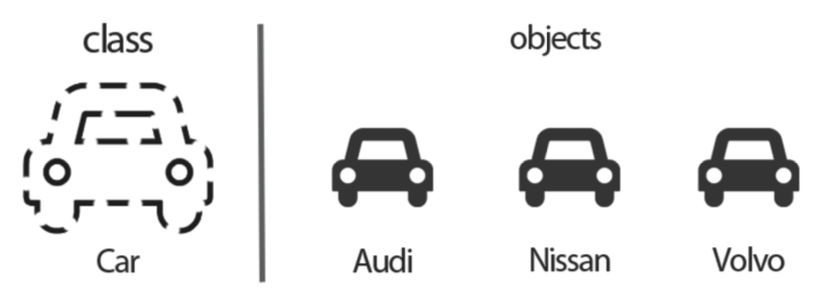
\includegraphics[width=\textwidth]{Figures/Screenshot 2021-11-08 at 4.10.55 PM}
	\caption{Class vs. Object(s)}
\end{figure}
Where possible methods may include:
\begin{itemize}
	\item steer left
	\item steer right
	\item brake
	\item ...
\end{itemize}
\vfill
\end{frame}
% -----------------------------------------------------------------------------
\section{Classes}
\subsection{Defining a Class}
\begin{frame}{Classes}
\vfill
Like function definitions begin with the \texttt{def} keyword in Python, class definitions begin with the \texttt{class} keyword.
\begin{table}[]
\begin{flushleft}
\begin{tabular}{ll}
\texttt{class Person:} &  \\
\texttt{\qquad """ Docstring of the class """} &  \\
\texttt{\qquad \# place here all variables} &  \\
\texttt{\qquad age = 10} &  \\
\texttt{\qquad \# place here all methods} &  \\
\texttt{\qquad def greet(self):} &  \\
\texttt{\qquad\qquad print("Hello")} &  \\
\end{tabular}
\end{flushleft}
\end{table}
\vfill
As soon as we define a class, a new "class object" is created with the same name.\\
This special "class object" allows us to see the attributes of the class (variables and/or methods) and, of course, to create new objects for that class.
\vfill
\end{frame}
%
\begin{frame}
\vfill
We can therefore now create new objects for that class:
\begin{table}[]
\begin{flushleft}
\begin{tabular}{ll}
\texttt{>{}>{}> charlie = Person()} &  \# instantiation of a new object\\
\texttt{>{}>{}> print(type(charlie))} &  \\
\texttt{<class '\_\_main\_\_.Person'>} &  \\
\end{tabular}
\end{flushleft}
\end{table}
\vfill
And we can also access to its attributes (methods and/or variable) via the well-known dot notation.
\begin{table}[]
\begin{flushleft}
\begin{tabular}{ll}
\texttt{>{}>{}> print(charlie.age)} & \\
\texttt{10} &  \\
\texttt{>{}>{}> print(charlie.greet())} &  \\
\texttt{Hello!} &  \\
\end{tabular}
\end{flushleft}
\end{table}
\vfill
\begin{block}{Note}
Instantiating a new object is pretty much similar to calling a function.
\end{block}
\vfill
\end{frame}
%
\subsection{\texttt{self}}
\begin{frame}
\vfill
You may have noticed the \texttt{self} parameter in the function definition inside the class, namely:
\begin{table}[]
\begin{flushleft}
\begin{tabular}{ll}
\texttt{class Person:} &  \\
\texttt{\qquad ...} &  \\
\texttt{\qquad def greet(self):} &  \\
\texttt{\qquad\qquad print("Hello")} &  \\
\end{tabular}
\end{flushleft}
\end{table}
Yet, we called the method simply as \texttt{charlie.greet()} without any arguments.
\vfill
This is because, whenever an object calls its method, the object itself is passed as the first argument. So, saying
\begin{table}[]
\begin{flushleft}
\begin{tabular}{ll}
\texttt{charlie.greet()} &  \\
\end{tabular}
\end{flushleft}
\end{table}
translates into
\begin{table}[]
\begin{flushleft}
\begin{tabular}{ll}
\texttt{Person.greet(charlie)} &  \\
\end{tabular}
\end{flushleft}
\end{table}
\vfill
The first argument of a class method must be the object itself. This is conventionally called \texttt{self}.
\vfill
\end{frame}
%
\subsection{Constructor}
\begin{frame}
\vfill
Initialising an internal variable as we did before, namely:
\begin{table}[]
\begin{flushleft}
\begin{tabular}{ll}
\texttt{class Person:} &  \\
\texttt{\qquad age = 10} &  \\
\texttt{\qquad ...} &  \\
\end{tabular}
\end{flushleft}
\end{table}
is not very flexible.
\vfill
We can use a special function called \texttt{\_\_init\_\_()} which is called whenever a new object is instantiated.\\
Commonly, it is used to initialise the internal variables of an object.\\
In Object-Oriented-Programming, this is called a \textcolor{red}{constructor}.
\begin{table}[]
\begin{flushleft}
\begin{tabular}{ll}
\texttt{class Person:} &  \\
\texttt{\qquad def \_\_init\_\_(self, firstName, lastName, age, address=None):} &  \\
\texttt{\qquad\qquad self.first\_name = firstName} &  \\
\texttt{\qquad\qquad self.last\_name = lastName} &  \\
\texttt{\qquad\qquad self.address = address} &  \\
\texttt{\qquad\qquad self.age = age} &  \\
\end{tabular}
\end{flushleft}
\end{table}
\vfill
\end{frame}
%
\subsection{Complete Examples}
\begin{frame}
\vfill
\begin{table}[]
\begin{flushleft}
\begin{tabular}{ll}
\texttt{class Person:} &  \\
\texttt{\qquad def \_\_init\_\_(self, firstName, lastName, age=None, address=None):} &  \\
\texttt{\qquad\qquad self.first\_name = firstName} &  \\
\texttt{\qquad\qquad self.last\_name = lastName} &  \\
\texttt{\qquad\qquad self.address = address} &  \\
\texttt{\qquad\qquad self.age = age} &  \\
\texttt{\qquad def greet(self):} &  \\
\texttt{\qquad\qquad print("Hello!")} &  \\
\texttt{\qquad\qquad print("My name is", self.first\_name, self.last\_name)} &  \\
\texttt{\qquad\qquad print("I am", self.age, "years old")} &  \\
\texttt{\qquad\qquad print("I live in", self.address)} &  \\
\texttt{ } &  \\
\texttt{person1 = Person("Alessio", "Martino", 30, "Viale Romania")} &  \\
\texttt{person2 = Person("Giorgio", "Piccardo")} &  \\
\texttt{ } &  \\
\texttt{person1.greet()} &  \\
\texttt{person2.greet()} &  \\
\end{tabular}
\end{flushleft}
\end{table}
\vfill
\end{frame}
%
\begin{frame}
\vfill
\begin{block}{Note}
You can pass input parameters to methods as well.
\end{block}
\begin{table}[]
\begin{flushleft}
\begin{tabular}{ll}
\texttt{class Dog:} &  \\
\texttt{\qquad def \_\_init\_\_(self, name, age):} &  \\
\texttt{\qquad\qquad self.name = name} &  \\
\texttt{\qquad\qquad self.age = age} &  \\
\texttt{\qquad def description(self):} &  \\
\texttt{\qquad\qquad return self.name + " is " + str(self.age) + " years old"} &  \\
\texttt{\qquad def speak(self, sound):} &  \\
\texttt{\qquad\qquad return self.name + " says " + sound} &  \\
\texttt{ } &  \\
\texttt{miles = Dog("Miles", 4)} &  \\
\texttt{print(miles.description())} &  \\
\texttt{print(miles.speak("Woof Woof"))} &  \\
\texttt{print(miles.speak("Bow Wow"))} &  \\
\end{tabular}
\end{flushleft}
\end{table}
\vfill
\end{frame}
% -----------------------------------------------------------------------------
\section{Modifying Objects}
\begin{frame}{Modifying Objects}
\vfill
So far we have seen:
\begin{itemize}
	\item "static" classes, e.g. \texttt{Person}: we initialise it with some values and that's it;
	\item  "less static" classes, e.g. \texttt{Dog}: we initialise it with some values, but we can also change the behaviour of methods at run-time.
\end{itemize}
\vfill
Now, the big question is: can we change the inner variables of an object?
\vfill
Short answer? Yes.
\vfill
\end{frame}
%
\begin{frame}
\vfill
\underline{Example}: let's define a data type to count events.\\
Think for example of a physical object, with a button: every time you press the button, the counter increases by 1\footnote{Such counter clicker machines exist: they are used to count e.g. cars passing on a road.}.
\vfill
How can we model it?
\begin{itemize}
	\item The \textit{domain} of our data type is the set of natural numbers
	\item The \textit{constant} is 0 (i.e., a counter that has not counted anything yet)
	\item The \textit{operations} are:
	\begin{itemize}
	\item \texttt{\_\_init\_\_()}, which initialises the counter to 0 (i.e., a brand new counter)
	\item \texttt{increase()}, which increases the counter by 1
	\item \texttt{get\_count()}, which reads the counter (i.e., returns the current count)
	\end{itemize}
\end{itemize}
\vfill
In order to represent the domain value (i.e., the counter internal state) we define a variable called \texttt{\_count}.
\begin{block}{Note}
The leading underscore conventionally states that it is an "internal", private variable of each instance.
\end{block}
\vfill
\end{frame}
%
\begin{frame}
\vfill
\begin{table}[]
\begin{flushleft}
\begin{tabular}{ll}
\texttt{class Counter:} &  \\
\texttt{\qquad def \_\_init\_\_(self):} & \\
\texttt{\qquad\qquad self.\_count = 0} & \\
\texttt{\qquad def increase(self):} & \\
\texttt{\qquad\qquad self.\_count += 1} & \\
\texttt{\qquad def get\_count(self):} & \\
\texttt{\qquad\qquad return self.\_count} & \\
\end{tabular}
\end{flushleft}
\end{table}
\vfill
\begin{block}{Recall}
Methods are defined exactly like ordinary functions, but inside the \texttt{class} block:
\begin{itemize}
	\item they can have any number of parameters
	\item the first parameter, that by convention is called \texttt{self}, has a special meaning as it contains a reference to the instance.
\end{itemize}
\end{block}
\begin{block}{Recall}
As \texttt{self} refers to the instance, we can access its variables via \texttt{self.<variable>}.
\end{block}
\vfill
\end{frame}
%
\begin{frame}
\vfill
And here's how to use it:
\begin{table}[]
\begin{flushleft}
\begin{tabular}{ll}
\texttt{c = Counter()} &  \hfill \qquad \qquad \qquad line 1\\
\texttt{c.increase()} &  \hfill line 2\\
\texttt{c.increase()} &  \hfill line 3\\
\texttt{state = c.get\_count()} &  \hfill line 4\\
\texttt{print("I have counted", state, "times")} &  \hfill line 5\\
\end{tabular}
\end{flushleft}
\end{table}
\vfill
What's going on here?
\begin{enumerate}
	\item on line 1, we create a new \texttt{Counter()} object. Instantiation automatically calls the \texttt{\_\_init\_\_()} method, which initialises the \texttt{\_count} variable to \texttt{0}
	\item on line 2, we trigger the \texttt{increase()} method, which increments \texttt{c.\_counter} by 1
	\item on line 3, we trigger the \texttt{increase()} method, which increments \texttt{c.\_counter} by 1
	\item on lines 4 and 5, we trigger the \texttt{get\_count()} method, which returns the current state of the counter (i.e., \texttt{c.\_counter}) and then we print it
\end{enumerate}
\vfill
\end{frame}
%
\subsection{Encapsulation}
\begin{frame}
\vfill
\begin{block}{Note}
We may as well increase \texttt{c.\_counter} by hand, like so:\\
\texttt{>{}>{}> c.\_counter += 1}\\
instead of calling \texttt{c.increase()}.\\
\vspace{2mm}
Can we do it? Yes.\\
Should we do it? No.
\end{block}
\vfill
Why? Because we seek to separate:
\begin{itemize}
	\item a public interface of the class, well described to the end-users via its methods by which we can manipulate objects;
	\item the inner working of the class, which is private to the class designer and should not be seen (or changed) from "outside of the box".
\end{itemize}
\vfill
This principle is known as \textcolor{red}{encapsulation}.
\vfill
\end{frame}
%
\begin{frame}
\vfill
Encapsulation works in the physical world too!
\begin{block}{Example}
You can use a car by manipulating its public interfaces (pedals, steering wheel, handbrake, ...) -- which are mostly standardised across models.\\
\vspace{2mm}
You do not have (and you probably do not want to) access internal parts of your car to operate it!
\end{block}
\vfill
Python, unlike other programming languages, does not forbid the end-user to access private attributes (which by convention begin with a \texttt{\_}).\\
\vfill
If you with to make it more difficult (but not impossible) to access to a private attribute, use double-underscores \texttt{\_\_}.
\vfill
\end{frame}
%------------------------------------------------------------------------------
\section{Inheritance}
\begin{frame}{Inheritance}
\vfill
\textcolor{red}{Inheritance} refers to defining a new class with little or no modification to an existing class:
\begin{itemize}
	\item the new class is called \textit{derived class} (or \textit{child class});
	\item the one from which it inherits is called the \textit{base class} (or \textit{parent class}).
\end{itemize}
\vfill
\vspace{2mm}
For the next example, recall the \texttt{Person} class:
\vspace{-3mm}
\begin{table}[]
\begin{flushleft}
\begin{tabular}{ll}
\texttt{class Person:} &  \\
\texttt{\qquad def \_\_init\_\_(self, firstName, lastName, age=None, address=None):} &  \\
\texttt{\qquad\qquad self.first\_name = firstName} &  \\
\texttt{\qquad\qquad self.last\_name = lastName} &  \\
\texttt{\qquad\qquad self.address = address} &  \\
\texttt{\qquad\qquad self.age = age} &  \\
\texttt{\qquad def greet(self):} &  \\
\texttt{\qquad\qquad print("Hello!")} &  \\
\texttt{\qquad\qquad print("My name is", self.first\_name, self.last\_name)} &  \\
\texttt{\qquad\qquad print("I am", self.age, "years old")} &  \\
\texttt{\qquad\qquad print("I live in", self.address)} &  \\
\end{tabular}
\end{flushleft}
\end{table}
\vfill
\end{frame}
%
\begin{frame}
\vfill
\underline{Example}: we want to create a class \texttt{Student} to represent university students. We want to represent data such as the student ID, the university name and the average grade using instance variables.
\begin{block}{Note}
But a student has also a last name, a first name, etc., like any person; because a student is a person! Name, surname, age and address are already available in the \texttt{Person} class.\\
\vspace{2mm}
Can we reinvent the wheel? Yes.\\
Should we do it? Nah.
\end{block}
We would like to define class \texttt{Student}, so that the following property holds:\\
\begin{center}Every instance of class \texttt{Student} is also an instance of class \texttt{Person}.\end{center}
In other words, we have detected an \underline{is-a} relation between students and persons (because \textit{a student is-a person}), and we would like to model this relation in our Python program.
\vfill
\end{frame}
%
\begin{frame}
\vfill
In Python is-a relations come to life thanks to inheritance. Let's define a class \texttt{Student} that extends class \texttt{Person}:
\begin{table}[]
\begin{flushleft}
\begin{tabular}{ll}
\texttt{class Student(Person):} &  \\
\texttt{\qquad pass} \qquad \qquad \# \texttt{pass} is a Python keyword that means "do nothing" & \\
\texttt{student1 = Student("Alessio", "Martino", 30, "Viale Romania")} &  \\
\texttt{print(student1.last\_name)} &  \\
\texttt{student1.greet()} &  \\
\texttt{print(type(student1))} &  \\
\end{tabular}
\end{flushleft}
\end{table}
\vfill
What's going on here?
\begin{itemize}
	\item \texttt{Person} is known as parent class of \texttt{Student}. As such, every instance of class \texttt{Student} inherits methods and instance variables from its parent class.
\end{itemize}
\begin{block}{Note}
You can inherit from multiple classes, e.g.:\\
\qquad \texttt{UniversityTeamPlayer(Student, Athlete)}\\
every instance of \texttt{UniversityTeamPlayer} inherits from \texttt{Student} and \texttt{Athlete}.\\
This is a slightly more advanced topic, yet it's good to know.
\end{block}
\vfill
\end{frame}
%
\begin{frame}
\vfill
\begin{block}{Hint}
You can surely use the \texttt{type()} function to check the class of an object. A clever alternative, which accounts for inheritance, is the \texttt{isinstance()} function.
\end{block}
The \texttt{isinstance(obj, c)} function is a predicate that tests whether an object \texttt{obj} is an instance of class \texttt{c}:
\begin{table}[]
\begin{flushleft}
\begin{tabular}{ll}
\texttt{Mary = Person('Stuart', 'Mary', 50)} &  \\
\texttt{Mark = Student('Holleymore', 'Mark', 22)} & \\
\texttt{print(isinstance(Mary, Person))} & \# yields \texttt{True} \\
\texttt{print(isinstance(Mary, Student))} & \# yields \texttt{False} \\
\texttt{print(isinstance(Mark, Person))} & \# yields \texttt{True} \\
\texttt{print(isinstance(Mark, Student))} & \# yields \texttt{True} \\
\end{tabular}
\end{flushleft}
\end{table}
\vfill
What's going on here?
\begin{itemize}
	\item we defined \texttt{Mary} as a \texttt{Person}, so she is not a \texttt{Student}
	\item we defined \texttt{Mark} as a \texttt{Student}, but a student is a person, so both of his \texttt{isinstance()} calls yield \texttt{True}
\end{itemize}
\vfill
\end{frame}
%
\begin{frame}
\vfill
\begin{block}{Problem}
There is still no difference between \texttt{Student} and \texttt{Person}.
\end{block}
Indeed, we still have to enrich the class \texttt{Student} in order to accomodate student ID, university name and grades.
\begin{table}[]
\begin{flushleft}
\begin{tabular}{ll}
\texttt{class Student(Person):} &  \\
\texttt{\quad def \_\_init\_\_(self,name,surname,uni,studID,age=None,addr=None):}& \\
\texttt{\quad\quad Person.\_\_init\_\_(self,name,surname,age,addr)}& \\
\texttt{\quad\quad self.university = uni}& \\
\texttt{\quad\quad self.studentID = studID}& \\
\texttt{\quad\quad self.exam\_grades = []}& \\
\texttt{ } &  \\
\texttt{\quad def add\_exam(self,grade):}& \\
\texttt{\quad\quad self.exam\_grades.append(grade)}& \\
\texttt{\quad def get\_average(self):}& \\
\texttt{\quad\quad return sum(self.exam\_grades) / len(self.exam\_grades)}& \\
\end{tabular}
\end{flushleft}
\end{table}
\vfill
\end{frame}
%
\begin{frame}
\vfill
What's going on here?
\begin{itemize}
	\item \texttt{Student} has a new \texttt{\_\_init\_\_()} that overwrites the one in \texttt{Person}
	\item when initialising \texttt{Student}, some input arguments that are proper to \texttt{Person} are fed to \texttt{Person.\_\_init\_\_()} so we can re-use its \texttt{\_\_init\_\_()}
	\item \texttt{Student} is initialised with two additional variables in order to account for the university name (\texttt{uni}) and the student ID (\texttt{studID})
	\item \texttt{Student} also features a third variable (\texttt{exam\_grades}) that collects the grades in a list
	\item \texttt{Student} also features two dedicated methods:
	\begin{enumerate}
		\item \texttt{add\_exam()} to add grades to the student's curriculum
		\item \texttt{get\_average()} to calculate the average student grade
	\end{enumerate}
\end{itemize}
\begin{block}{Warning}
The is-a relation is a one-way relation: in our case, all students are persons, but not all persons are students.\\
Practically speaking, \texttt{Student} inherits from \texttt{Person}, but \texttt{Person} does not inherit from \texttt{Student}.
\end{block}
\vfill
\end{frame}
%
\begin{frame}
\vfill
Let's see our brand new \texttt{Student} class in action.
\begin{table}[]
\begin{flushleft}
\begin{tabular}{ll}
\texttt{student1 = Student("Alessio", "Martino", ... } &  \\
\texttt{\ \ \ \ \ \ \ \ \ \ \ \ \ \ "LUISS", "123456", 30, "Viale Romania")} &  \\
\texttt{ } &  \\
\# what we inherited from \texttt{Person} &  \\
\texttt{print(student1.first\_name)} \qquad \# prints \texttt{Alessio}&\\
\texttt{student1.greet()} \qquad\quad\quad\quad\quad \ \ \# prints \texttt{Hello! My name is ...} & \\
\texttt{ } &  \\
\# what we defined in \texttt{Student} &  \\
\texttt{student1.add\_exam(30)} \qquad \# we have \texttt{student1.exam\_grades = [30]} &  \\
\texttt{student1.add\_exam(25)} \qquad \# we have \texttt{student1.exam\_grades = [30, 25]} &  \\
\texttt{student1.add\_exam(18)} \qquad \# we have \texttt{student1.exam\_grades = [30, 25, 18]} &  \\
\texttt{print(student1.get\_average())} \quad \# prints \texttt{24.333333333} &  \\
\end{tabular}
\end{flushleft}
\end{table}
\vfill
\end{frame}
%------------------------------------------------------------------------------
\section{Polymorphism}
\begin{frame}{Polymorphism}
\vfill
\begin{block}{Note}
In the child class you can overwrite any methods, not just \texttt{\_\_init\_\_()}.
\end{block}
\vfill
This aspect introduces us to the concept of \textcolor{red}{polymorphism}.
\vfill
Broadly speaking, in computer programming, polymorphism means the same function name (but different signatures) being used for different types.
\vfill
In Python, common polymorphic functions include:
\begin{itemize}
	\item \texttt{len()}, that returns the number of characters in a string, the number of items in a tuple/list, the number of key-value pairs in a dictionary
	\item \texttt{sum()}, which adds the elements of a sequence as long as the elements of the sequence support addition.
\end{itemize}
\vfill
\end{frame}
%
\begin{frame}
Let's suppose that our \texttt{greet()} does not look nice in the context of a university student.\\
In its "standard form" (i.e., derived from the \texttt{Person} class), it reads as
\begin{table}[]
\begin{flushleft}
\begin{tabular}{ll}
\texttt{def greet(self):} &  \\
\texttt{\qquad print("Hello!")} &  \\
\texttt{\qquad print("My name is", self.first\_name, self.last\_name)} &  \\
\texttt{\qquad print("I am", self.age, "years old")} &  \\
\texttt{\qquad print("I live in", self.address)} &  \\
\end{tabular}
\end{flushleft}
\end{table}
Inside the \texttt{Student} class, we can re-define \texttt{greet()} with something like:
\begin{table}[]
\begin{flushleft}
\begin{tabular}{ll}
\texttt{def greet(self):} &  \\
\texttt{\qquad print("Hello!")} &  \\
\texttt{\qquad print("My name is", self.first\_name, self.last\_name)} &  \\
\texttt{\qquad print("I am a student at", self.university)} &  \\
\texttt{\qquad print("My average grade is", self.get\_average())} &  \\
\end{tabular}
\end{flushleft}
\end{table}
\begin{block}{Note}
This is a particular type of polymorphism known as \textit{method overriding}.
\end{block}
\end{frame}
%
\begin{frame}
\vfill
The \texttt{greet()} inside \texttt{Student} overwrites the inherited one from \texttt{Person}.
\vfill
Indeed, we now have:
\begin{table}[]
\begin{flushleft}
\begin{tabular}{ll}
\texttt{student1 = Student("Alessio", "Martino", ... } &  \\
\texttt{\ \ \ \ \ \ \ \ \ \ \ \ \ \ "LUISS", "123456", 30, "Viale Romania")} &  \\
\texttt{student1.add\_exam(30)} \qquad \# we have \texttt{student1.exam\_grades = [30]} &  \\
\texttt{student1.add\_exam(25)} \qquad \# we have \texttt{student1.exam\_grades = [30, 25]} &  \\
\texttt{student1.add\_exam(18)} \qquad \# we have \texttt{student1.exam\_grades = [30, 25, 18]} &  \\
\texttt{student1.greet()} &  \\
\end{tabular}
\end{flushleft}
\end{table}
at it will print
\begin{table}[]
\begin{flushleft}
\begin{tabular}{ll}
\texttt{Hello!} &  \\
\texttt{My name is Alessio Martino} &  \\
\texttt{I am a student at LUISS} &  \\
\texttt{My average grade is 24.333333333333332} &  \\
\end{tabular}
\end{flushleft}
\end{table}
\vfill
\end{frame}
%
\begin{frame}
\vfill
Due to polymorphism, the Python interpreter automatically recognises that the \texttt{greet()} method has been overwritten in the child class. So, it uses the one defined in the child class.
\vfill
As instead, for objects pertaining to the parent class, the \texttt{greet()} method remains untouched.
\vfill
What does this code do?
\vspace{-2mm}
\begin{table}[]
\begin{flushleft}
\begin{tabular}{ll}
\texttt{student1 = Student("Alessio", "Martino", ... } &  \\
\texttt{\ \ \ \ \ \ \ \ \ \ \ \ \ \ "LUISS", "123456", 30, "Viale Romania")} &  \\
\texttt{student1.add\_exam(30)} \qquad \# we have \texttt{student1.exam\_grades = [30]} &  \\
\texttt{student1.add\_exam(25)} \qquad \# we have \texttt{student1.exam\_grades = [30, 25]} &  \\
\texttt{student1.add\_exam(18)} \qquad \# we have \texttt{student1.exam\_grades = [30, 25, 18]} &  \\
\texttt{person1 = Person("Giorgio", "Piccardo")} &  \\
\texttt{list\_of\_persons = [student1, person1]} &  \\
\texttt{for item in list\_of\_persons:} &  \\
\texttt{\qquad item.greet()} &  \\
\end{tabular}
\end{flushleft}
\end{table}
\vfill
\end{frame}
%------------------------------------------------------------------------------
%\section{References}
%\begin{frame}[allowframebreaks]{References}
%%\bibliographystyle{apacite}
%\printbibliography[heading=none]
%\end{frame}
\section{References}
\begin{frame}{References}
\begin{itemize}
	\item Guttag, J. V. (2013). \textit{Introduction to Computation and Programming using Python (Revised and Expanded Edition)}. MIT Press. [Chapter 8 -- no 8.3.1 and later]
	\item Downey, A. (2015). \textit{Think Python}. Green Tea Press ed. 2nd. [Sections 15.1, 15.2, 15.5, 15.6, 16.2, 16.3, 17.1, 17.5, 17.9]
\end{itemize}
\end{frame}
%------------------------------------------------------------------------------
\section{Acknowledgments}
\begin{frame}{Acknowledgments}
% \begin{itemize}
% 	\item Prof. Irene Finocchi (LUISS University)\\
% 	\quad \textit{Introduction to Computer Programming} Lecture Notes (2020-2021)
% \end{itemize}
\end{frame}
%------------------------------------------------------------------------------
%\subsection{Sites legais}
%\begin{frame}{Sites legais}
%  Want to know more? See!
%  \begin{itemize}
%    \item Browse in my page \url{http://www.ezefranca.com}.
%    \item Browse on BCC page \url{http://www.sp.senac.br/bcc}.
%    \item Thanks WriteLaTeX from Support! \url{http://www.writelatex.com}.
%  \end{itemize}
%
%\end{frame}
%------------------------------------------------------------------------------

% -----------------------------------------------------------------------------
\end{document}
%-----------------------------------------------Este comentario nunca aparecera
